Für eine eventuelle BIAS-Korrektur kommt eine bisherige Herangehensweise nicht in Frage, da dadurch die lokale und vor allem zeitliche Varianz zu stark beeinträchtigt wird wie in Abb. \ref{fig:boxplot_corrected_rcp} zu erkennen ist. Laut D.Maraun \cite{biasMaraun} ist dafür ein Herangehensweise über stochastische Quantile-Mapping nötig. Dabei ist vor allem auf Überkorrektur acht zu geben, welche sich durch die Überschätzung der Flächenmittelwerte für Extremniederschläge und falsche Trends äußert. Die von Maraun in \cite{biasMaraun} postulierte Herangehensweise wird in diesem Kapitel verfolgt.
\section{Herangehensweise}
\begin{itemize}
	\item Zunächst wurden die am stärksten von Abweichungen betroffenen Regionen ausgemacht. Dies erfolgte über die Jahreszeiten bzw. Monate.
	\item Als nächster Schritt werden die Jahreszeiten einzeln betrachtet, da in ihnen typische Korrelationen herrschen.
\end{itemize}

\section{Am stärksten abweichende Regionen}
Die betreffenden Datensätze (historical, evaluation und APGD) wurden zunächst in monatliche Abschnitte unterteilt. Diese wurden dann einer Quantil-Berechnung über alle Jahre unterzogen. In Folge wurden die 20 größten und 20 kleinsten Abweichungen von den entsprechenden Quantilen des Beobachtungsdatensatzes den Monaten entsprechend auf einer Karte abgebildet um die am stärksten betroffenen Regionen zu erkennen.\\
Wie man in Abb.\ref{fig:decision_plot_q99-eval} erkennen kann befindet sich in der südöstlichen Region (um die Stadt Split) eine Zone, die extreme Abweichungen im 99.Quantil über alle Monate zeigt, dies deutet sich bereits in der Abbildung des 90. Quantils ab (Abb. \ref{fig:decision_plot_q90-eval}). Um die Darstellung zu verbessern und die Ausreißer zu minimieren wird diese Region zunächst aus den folgenden Berechnungen ausgeschnitten und außen vor gelassen. Die plots mit den ausgeschnittenen Ausreißer-Bereichen sind in Abb. \ref{fig:cropped_decision_plot_q90-hist}-\ref{fig:cropped_decision_plot_q99-eval} abgebildet. Die in Rechtecken gekennzeichneten Regionen werden in Folge näher betrachtet, da in ihnen die größten Abweichungen herrschen und sie konstant über die Monate einer Jahreszeit verteilt sind. Man erkennt im Vergleich der plots für das 90. Quantil des evaluation-Datensatzes und des historical-Datensatzes, dass die gekennzeichneten Regionen großteils an der selben Stelle sind. Diese werden für die folgenden Berechnungen zusammengelegt und ihre verschiedenen Positionen überlappt.\\
Für das 99. Quantil der beiden Datensätze herrscht leider keine solche allgemeine Übereinstimmung der Positionen für die maximalen Abweichungen (siehe Abb. \ref{fig:cropped_decision_plot_q99-hist} und Abb. \ref{fig:cropped_decision_plot_q99-eval}). Nur ein Teil der maximalen Abweichungen im Winter und im Frühling sind an derselben Stelle. Deshalb werden für das 99. Quantil nur diese beiden Jahreszeiten weiter betrachtet, da sonst eine zu große Region betrachtet werden müsste, was die Aussagekraft der folgenden Berechnungen stark einschränken würde, beziehungsweise diese zu Unübersichtlich machen würde.


\begin{figure}[h!]
	\centering{
	\begin{subfigure}{0.49\textwidth}
		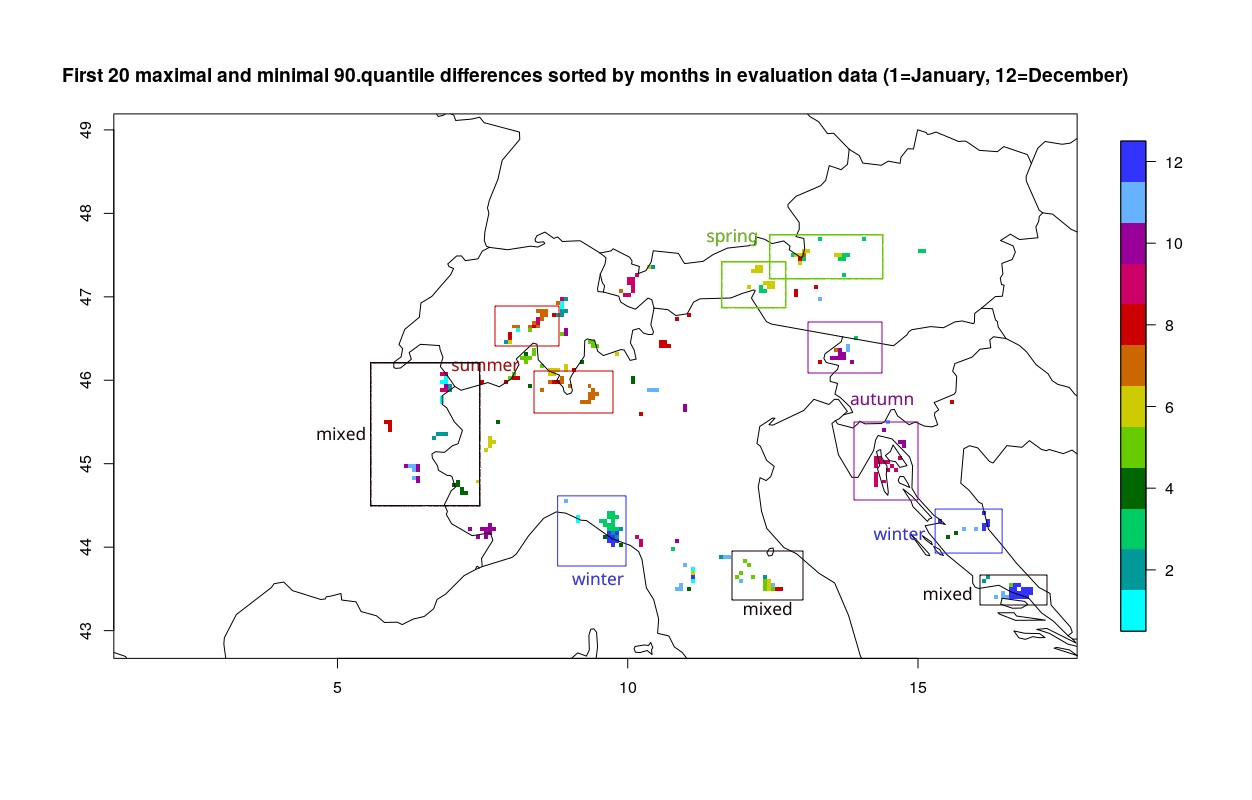
\includegraphics[width=\textwidth]{/quantile/decision_plot_q90-eval.png}
		\caption{Die 40 größten Abweichungen im 90.Quantil des evaluation-Datensatzes.}
		\label{fig:decision_plot_q90-eval}
	\end{subfigure}
	\begin{subfigure}{0.49\textwidth}
		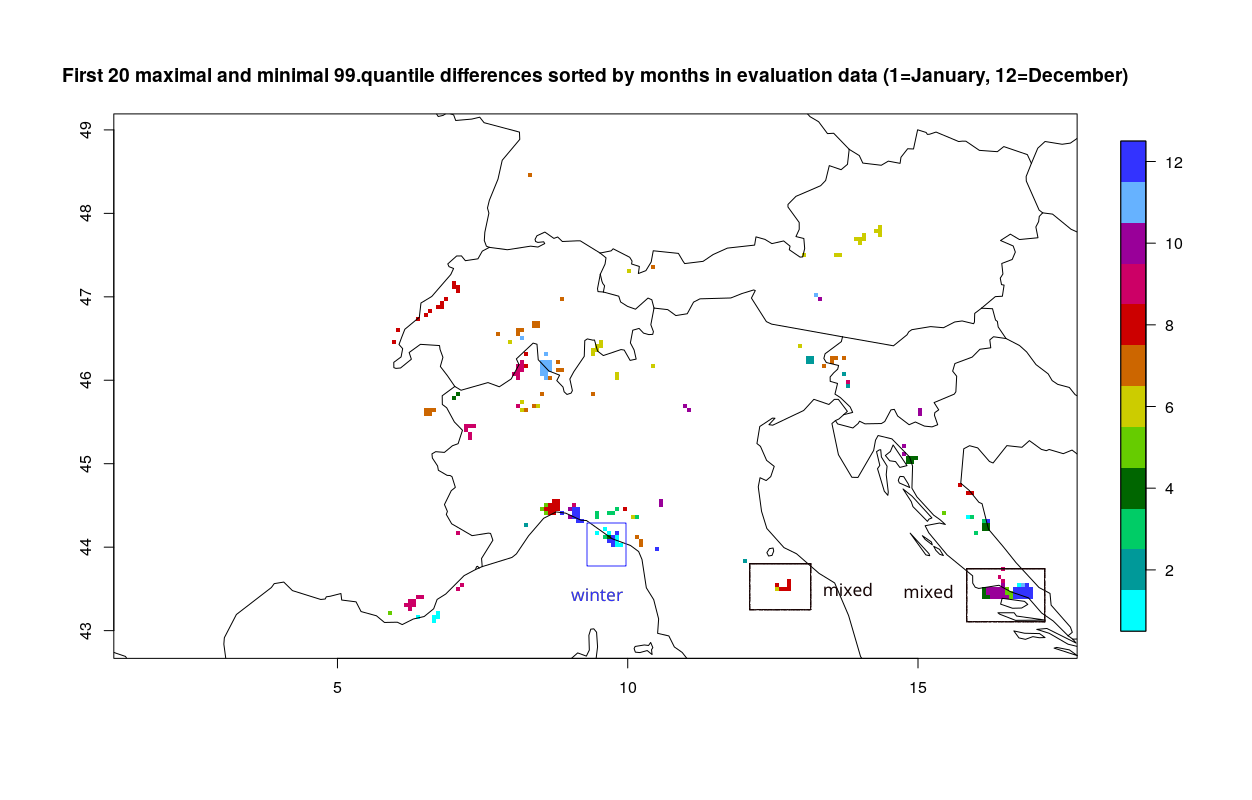
\includegraphics[width=\textwidth]{/quantile/decision_plot_q99-eval.png}
		\caption{Die 40 größten Abweichungen im 99.Quantil des evaluation-Datensatzes.}
		\label{fig:decision_plot_q99-eval}
	\end{subfigure}
	\caption{Abbildungen zur Illustration des Ausreißer-Bereichs, zu sehen im süd-östlichen Eck.}
}
\end{figure}
\begin{figure}[h!]
	\centering{
		\begin{subfigure}{0.47\textwidth}
			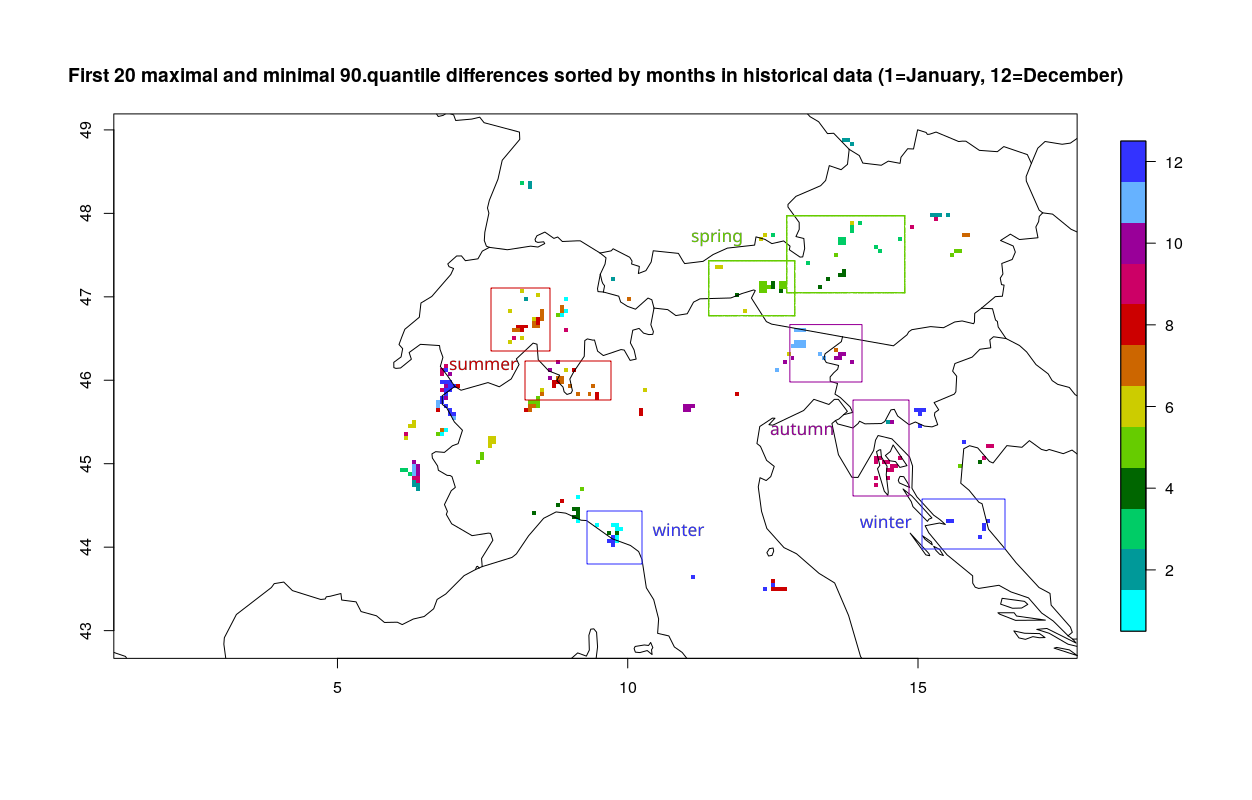
\includegraphics[angle=270, width=\textwidth]{/quantile/cropped_decision_q90-hist.png}
			\caption{Die 40 größten Abweichungen im 90.Quantil des historical-Datensatzes mit ausgeschnittenem Ausreißern.}
			\label{fig:cropped_decision_plot_q90-hist}
		\end{subfigure}
		\begin{subfigure}{0.47\textwidth}
			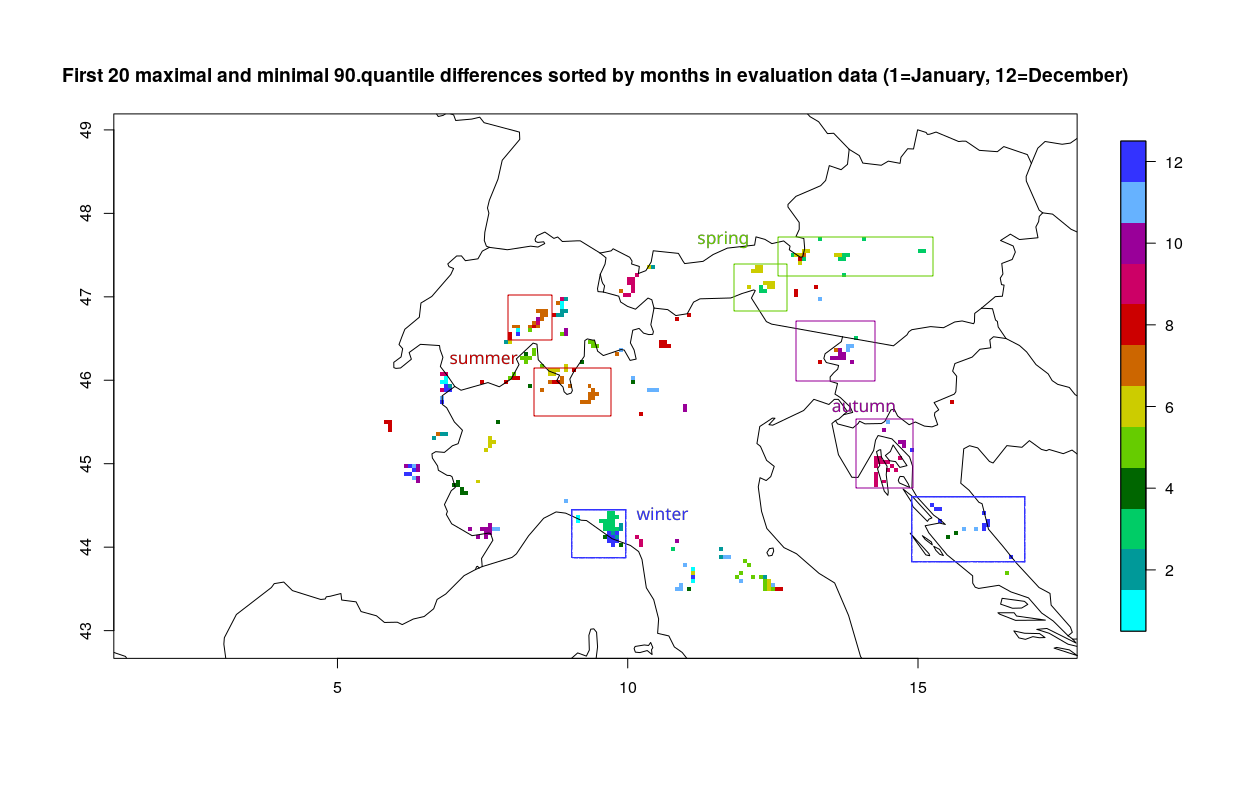
\includegraphics[angle=270, width=\textwidth]{/quantile/cropped_decision_q90-eval.png}
			\caption{Die 40 größten Abweichungen im 90.Quantil des evaluation-Datensatzes mit ausgeschnittenem Ausreißern.}
			\label{fig:cropped_decision_plot_q90-eval}
		\end{subfigure}
		\begin{subfigure}{0.47\textwidth}
			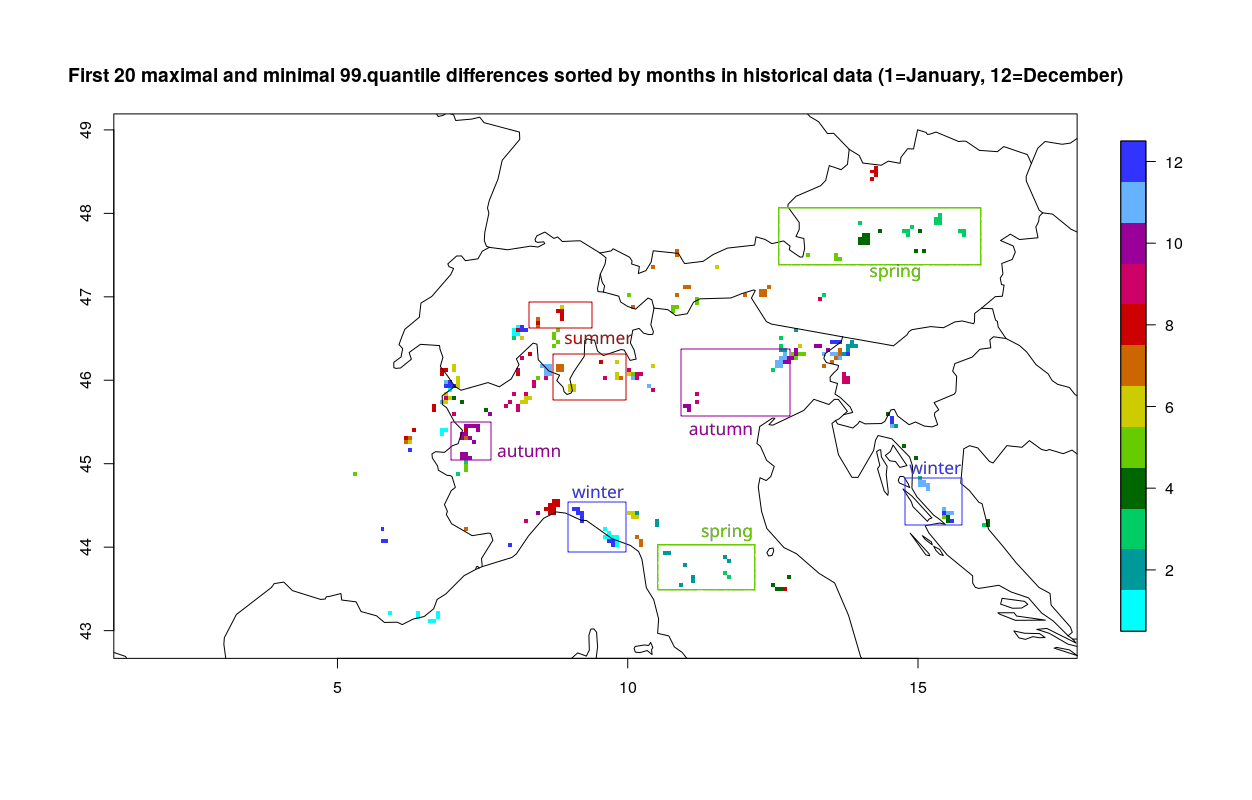
\includegraphics[angle=270, width=\textwidth]{/quantile/cropped_decision_q99-hist.png}
			\caption{Die 40 größten Abweichungen im 99.Quantil des historical-Datensatzes mit ausgeschnittenem Ausreißern.}
			\label{fig:cropped_decision_plot_q99-hist}
		\end{subfigure}
		\begin{subfigure}{0.47\textwidth}
			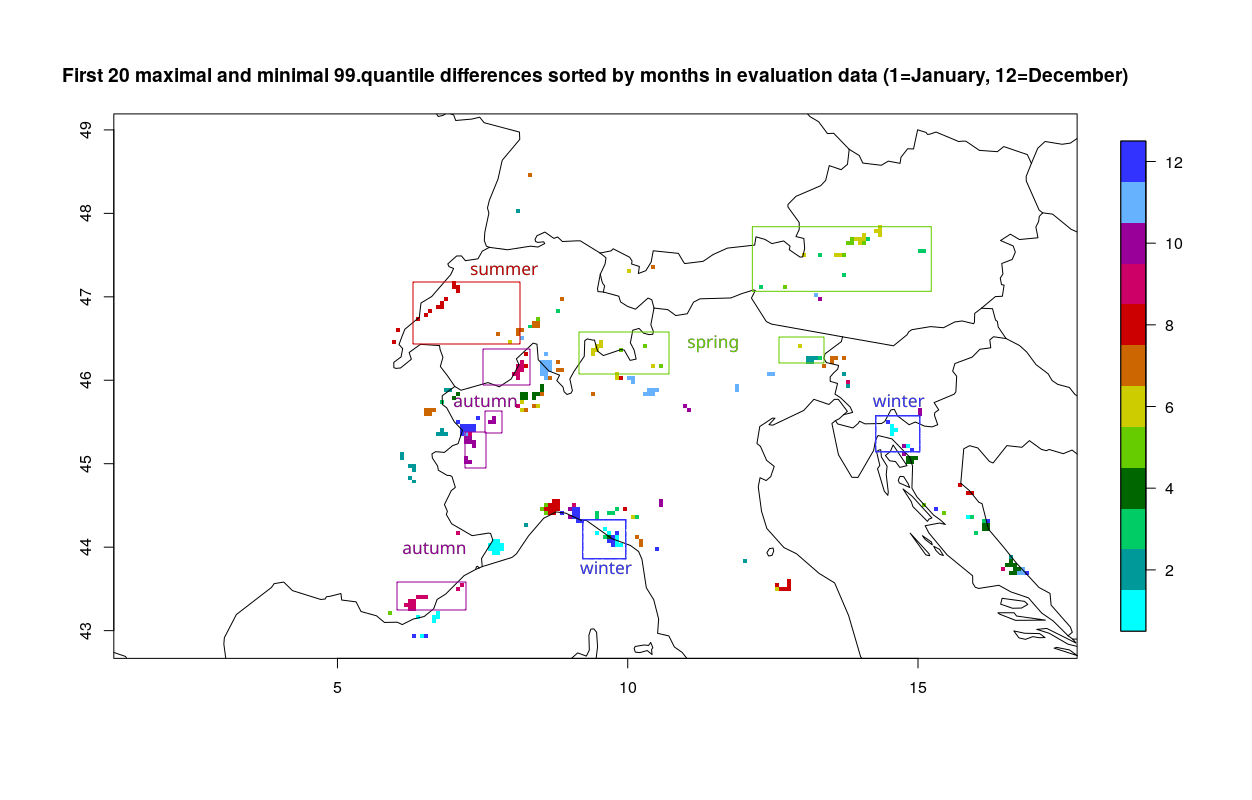
\includegraphics[angle=270, width=\textwidth]{/quantile/cropped_decision_q99-eval.png}
			\caption{Die 40 größten Abweichungen im 99.Quantil des evaluation-Datensatzes mit ausgeschnittenem Ausreißern.}
			\label{fig:cropped_decision_plot_q99-eval}
		\end{subfigure}
	}
\end{figure}

\section{Frühling}
